%%%%%%%%%%%%%%%%%%%%%%%%%%%%%%%%%%%%%%%%%
% Short Sectioned Assignment LaTeX Template Version 1.0 (5/5/12)
% This template has been downloaded from: http://www.LaTeXTemplates.com
% Original author:  Frits Wenneker (http://www.howtotex.com)
% License: CC BY-NC-SA 3.0 (http://creativecommons.org/licenses/by-nc-sa/3.0/)
%%%%%%%%%%%%%%%%%%%%%%%%%%%%%%%%%%%%%%%%%

% !TEX root = ./proyecto.tex

% \documentclass[paper=a4, fontsize=11pt]{scrartcl} % A4 paper and 11pt font size
\documentclass[11pt, a4paper]{book}
\usepackage[T1]{fontenc} % Use 8-bit encoding that has 256 glyphs
\usepackage[utf8]{inputenc}
%\usepackage{fourier} % Use the Adobe Utopia font for the document - comment this line to return to the LaTeX default
\usepackage{listings} % para insertar código con formato similar al editor
\usepackage[spanish, es-tabla]{babel} % Selecciona el español para palabras introducidas automáticamente, p.ej. "septiembre" en la fecha y especifica que se use la palabra Tabla en vez de Cuadro
\usepackage{url} % ,href} %para incluir URLs e hipervínculos dentro del texto (aunque hay que instalar href)
\usepackage{graphics,graphicx, float} %para incluir imágenes y colocarlas
\usepackage[gen]{eurosym} %para incluir el símbolo del euro
\usepackage{cite} %para incluir citas del archivo <nombre>.bib
\usepackage{enumerate}
\usepackage{hyperref}
\usepackage{graphicx}
\usepackage{tabularx}
\usepackage{booktabs}
\usepackage{ragged2e}

\usepackage{baskervillef}
\usepackage[varqu,varl,var0]{inconsolata}
\usepackage[scale=.95,type1]{cabin}
\usepackage[baskerville,vvarbb]{newtxmath}
\usepackage[cal=boondoxo]{mathalfa}

\usepackage[table,xcdraw]{xcolor}
\hypersetup{
	colorlinks=true,	% false: boxed links; true: colored links
	linkcolor=black,	% color of internal links
	urlcolor=cyan		% color of external links
}
\renewcommand{\familydefault}{\rmdefault}
\usepackage{fancyhdr} % Custom headers and footers
\pagestyle{fancyplain} % Makes all pages in the document conform to the custom headers and footers
\fancyhead[L]{} % Empty left header
\fancyhead[C]{} % Empty center header
\fancyhead[R]{Miguel Pedregosa Pérez} % My name
\fancyfoot[L]{} % Empty left footer
\fancyfoot[C]{} % Empty center footer
\fancyfoot[R]{\thepage} % Page numbering for right footer
\renewcommand{\footrulewidth}{0pt} % Remove footer underlines
\setlength{\headheight}{13.6pt} % Customize the height of the header

\usepackage{titlesec, blindtext, color}
\definecolor{gray75}{gray}{0.75}
\newcommand{\hsp}{\hspace{20pt}}
\titleformat{\chapter}[hang]{\Huge\rmfamily\bfseries}{\thechapter\hsp\textcolor{gray75}{|}\hsp}{0pt}{\Huge\rmfamily\bfseries}
\setcounter{secnumdepth}{4}
\usepackage[Lenny]{fncychap}
%\usepackage[indent=0.5cm, skip=6pt]{parskip}

\usepackage{caption}
\usepackage{subcaption}

\definecolor{dkgreen}{rgb}{0,0.6,0}
\definecolor{dred}{rgb}{0.545,0,0}
\definecolor{dblue}{rgb}{0,0,0.545}
\definecolor{lgrey}{rgb}{0.95,0.95,0.95}
\definecolor{gray}{rgb}{0.4,0.4,0.4}
\definecolor{darkblue}{rgb}{0.0,0.0,0.6}
\lstdefinelanguage{cpp}{
      backgroundcolor=\color{lgrey},  
      basicstyle=\footnotesize \ttfamily \color{black} \bfseries,
      breakatwhitespace=false,       
      breaklines=true,               
      captionpos=b,                   
      commentstyle=\color{dkgreen},   
      deletekeywords={...},          
      escapeinside={\%*}{*)},                  
      frame=single,                  
      language=C++,                
      keywordstyle=\color{purple},  
      morekeywords={BRIEFDescriptorConfig,string,TiXmlNode,DetectorDescriptorConfigContainer,istringstream,cerr,exit}, 
      identifierstyle=\color{black},
      stringstyle=\color{blue},      
      numbers=right,                 
      numbersep=5pt,                  
      numberstyle=\tiny\color{black}, 
      rulecolor=\color{black},        
      showspaces=false,               
      showstringspaces=false,        
      showtabs=false,                
      stepnumber=1,                   
      tabsize=4,                     
      title=\lstname,                 
    }


\newcommand{\titulo}{Contribuciones a GenoMus}
\newcommand{\subtitulo}{Rediseño de un motor de cómputo funcional sobre estructuras musicales}
\newcommand{\autor}{Miguel Pedregosa Pérez}

\begin{document}

	% Plantilla portada UGR
	\begin{titlepage}
\newlength{\centeroffset}
\setlength{\centeroffset}{-0.5\oddsidemargin}
\addtolength{\centeroffset}{0.5\evensidemargin}
\thispagestyle{empty}

\noindent\hspace*{\centeroffset}\begin{minipage}{\textwidth}

\centering

\includegraphics[width=0.9\textwidth]{logos/logo_ugr.jpg}\\[1.4cm]

\textsc{ \Large TRABAJO FIN DE GRADO\\[0.2cm]}
\textsc{ GRADO EN INGENIERIA INFORMATICA}\\[1cm]

{\Huge\bfseries Título \\}
\noindent\rule[-1ex]{\textwidth}{3pt}\\[3.5ex]
{\large\bfseries Subtítulo }
\end{minipage}

\vspace{2.5cm}
\noindent\hspace*{\centeroffset}
\begin{minipage}{\textwidth}
\centering

\textbf{Autor}\\ {Estudiante}\\[2.5ex]
\textbf{Director}\\ {Tutor(a)(es)}\\[2cm]

\includegraphics[width=0.3\textwidth]{logos/etsiit_logo.png}\\[0.1cm]
\textsc{Escuela Técnica Superior de Ingenierías Informática y de Telecomunicación}\\
\textsc{---}\\
Granada, Junio de 201x
\end{minipage}
\end{titlepage}


	% Plantilla prefacio UGR
	\thispagestyle{empty}

\begin{center}
{\large\bfseries Título \\ Subtítulo }\\
\end{center}
\begin{center}
Nombre Del Estudiante\\
\end{center}

%\vspace{0.7cm}

\vspace{0.5cm}
\noindent\textbf{Palabras clave}: \textit{software libre}
\vspace{0.7cm}

\noindent\textbf{Resumen}\\
	

\cleardoublepage

\begin{center}
	{\large\bfseries Same, but in English}\\
\end{center}
\begin{center}
	Student's name\\
\end{center}
\vspace{0.5cm}
\noindent\textbf{Keywords}: \textit{open source}, \textit{floss}
\vspace{0.7cm}

\noindent\textbf{Abstract}\\


\cleardoublepage

\thispagestyle{empty}

\noindent\rule[-1ex]{\textwidth}{2pt}\\[4.5ex]

D. \textbf{Tutora/e(s)}, Profesor(a) del ...

\vspace{0.5cm}

\textbf{Informo:}

\vspace{0.5cm}

Que el presente trabajo, titulado \textit{\textbf{Chief}},
ha sido realizado bajo mi supervisión por \textbf{Estudiante}, y autorizo la defensa de dicho trabajo ante el tribunal
que corresponda.

\vspace{0.5cm}

Y para que conste, expiden y firman el presente informe en Granada a Junio de 2018.

\vspace{1cm}

\textbf{El/la director(a)/es: }

\vspace{5cm}

\noindent \textbf{(nombre completo tutor/a/es)}

\chapter*{Agradecimientos}






	% Índice de contenidos
	\newpage
	\tableofcontents

	% Índice de imágenes y tablas
	\newpage
	\listoffigures

	% Si hay suficientes se incluirá dicho índice
	\listoftables 
	\newpage

	% Introducción 
	\chapter{Introducción}

Este proyecto es software libre, y está liberado con la licencia \cite{gplv3}.
	
	% Estado del arte
	% 	1. Crítica al estado del arte
	% 	2. Propuesta
	\chapter{Estado del arte}


\begin{quote}
    [...] If a musician could ``jam'' with an unseen Jam Factory and with an unseen human musician for as long as desired and was unable to tell which was the human, than, according to the Turing test, Jam Factory would have exhibited ``intelligence''. \cite{musical_turing}
\end{quote}


Al igual que otros campos pertenecientes a las humanidades digitales, el estudio del fenómeno musical bajo la lente de la computación ha planteado diferentes cuestiones acerca de la creatividad artificial. La cuestión primigenia es la misma que en el resto de campos, y es equivalente a la cuestión formulada en el test de Turing: ¿puede una computadora replicar los comportamientos de un humano en el ámbito de la música? Dado que el abanico de prácticas musicales es amplio y diverso, esta pregunta requiere de especificación en los diferentes campos de computación musical. Proyectos como Magenta\footnote{Magenta es un proyecto de software libre perteneciente a Google que explora el rol de la inteligencia artifical en el proceso creativo. Más información en la página oficial (\url{https://magenta.tensorflow.org/}).} buscan el perfeccionamiento de la síntesis de sonido o material musical como proceso aislado. Otros proyectos como \textit{Piano Genie}\footnote{Más información en su página oficial \url{https://glitch.com/edit/\#!/piano-genie}} buscan la interactividad musical entre usuario y software.

GenoMus se enmarca en el campo de la CAC (Composición Asistida por Computadora), campo cuya búsqueda principal es la de proporcionar al artista (el compositor) una extensión de su propia creatividad a través del uso de técnicas de composición automática. Este campo cuenta con una larga historia (en la escala de la historia de la computación) con multitud de planteamientos, algunos de los cuales se intentan explicar brevemente a continuación.

\section{CAC a través de procesos matemáticos}

Las aproximaciones que caen bajo el paraguas del análisis de procesos matemáticos sobre estructuras musicales tienen en común la utilización de transformaciones matemáticas sobre datos musicales que muchas veces están representados con la nota musical como grano indivisible. Podemos encontrar ejemplos del tratamiento algorítmico del material musical, que lo traduce a otras instancias musicales.

En estas aproximaciones se introduce recurrentemente el concepto de \textit{música fractal}, instancias de música autosemejante procedentes de transformaciones algorítmicas de materiales musicales más simples. También podemos incluir en este grupo los trabajos realizados con autómatas celulares. Podemos ejemplificar este grupo con trabajo de Ninagawa\footnote{En el texto ``1/f Noise in Elementary Cellular Automaton Rule 110''\cite{Ninagawa}.} o de Richard French\cite{automata-repr}.

\section{CAC a través de gramáticas}

Estas aproximaciones tienen como elemento común la codificación de los procesos de composición usuales en gramáticas generativas. Este enfoque tiene una correspondencia directa con el análisis tradicional de la música, a través del cual se puede definir la música como un lenguaje describible por gramáticas no deterministas. Por ejemplo, la totalidad de la teoría armónica del periodo de la práctica común puede reducirse a un problema de combinatoria de datos musicales. No obstante, estas gramáticas están sujetos a movimientos o culturas musicales concretos, lo que hace muy difícil la obtención de una gramática que refleje fielmente la totalidad de procesos cognitivos que se dan en el fenómeno musical. En este campo podemos destacar el trabajo de F. Lerdahl y R. Jackendoff\cite{generative-theory}.

\section{Evaluación y retroalimentación}

La búsqueda de la extensión de la creatividad del compositor está abocada a la cooperación entre el sistema de composición automática elegido y las intenciones del compositor. Esto implica la necesidad de una evaluación estética por parte del usuario de los artificios del software utilizado, evaluación que se puede realizar de diferentes maneras. Desde la creación de productos basados en restricciones del compositor a través de algoritmos evolutivos hasta la propia modificación y aprendizaje del sistema generativo, esta interacción entre la evaluación del compositor y el sistema generador de música es lo que da valor estético o artístico al producto obtenido.

GenoMus plantea un proceso de definición de restricciones sobre material musical, del cual hace uso el software para proporcional al compositor de instancias de música deseadas\cite{GenoMus-master}. La calidad y usabilidad de este flujo de comunicación quedará directamente determinada por la potencia del motor de cómputo subyacente, el cual posibilitará o no la interacción a tiempo real entre el compositor y el programa.





	% Descripción del problema y hasta donde se llega
	\chapter{Descripción del problema}\label{cap:descripcion}

\section{Abstracción musical y metaprogramación}

La música tal y como la conocemos en nuestra sociedad es un fenómeno que se puede entender a través de la sucesiva construcción de lenguajes a diferentes niveles de abstracción sobre el fenómeno físico del sonido. A través del estudio de estos constructos sintácticos y semánticos podemos estudiar la respuesta cognitiva o emocional de las instancias de música en las personas. De esta misma manera, las instancias de música son describibles a cualquiera de estos niveles.

GenoMus propone un framework de metaprogramación musical, sustentado por un modelo de cómputo funcional sobre datos musicales, y originariamente implementado sobre javascript. El software define transformaciones musicales como la repetición, concatenación o transporte y es capaz de declarar estructuras de transformaciones sobre datos musicales que proporcionan nuevos datos musicales al evaluarse. Las transformaciones definidas por GenoMus posibilitan la descripción de música en un nivel de abstracción mayor que el del modelo de datos musicales que maneja.

\begin{table}[]
    \centering
    \begin{tabular}{l | l}
        \textbf{Nivel de abstracción} & \textbf{Conceptos medibles} \\ \hline \hline
        Nivel físico & Ondas, frecuencia, amplitud \\
        Nivel auditivo & Altura, timbre, intensidad, duración \\
        Nivel cognitivo & Notas, voces, forma \\
        Nivel cultural & Estilo, intención, emoción
    \end{tabular}
    \caption{Niveles de abstracción musical ordenados de menos a más abstracto.}
    \label{tab:abstraccion_musical}
\end{table}

El nivel de abstracción del modelo de datos musicales de GenoMus se corresponde con el nivel de abstracción que podemos ver en una representación usual de música destinada a la interpretación por un músico o por un instrumento virtual, es decir la representación de la música en términos de notas y voces. De esta manera, las instancias de datos musicales manejadas por GenoMus pueden ser fácilmente representables en formatos legibles por personas o instrumentos virtuales, como partituras o MIDI\footnote{El formato MIDI es un formato estandarizado de codificación de datos musicales. Más información en la especificación oficial de las diferentes versiones del estándar, consultables en \url{https://www.midi.org/specifications/file-format-specifications}}.

De esta manera, GenoMus es metaprogramación musical ya que declara estructuras de transformaciones musicales sobre datos musicales ya abstractos de por sí.

\section{Genotipos y fenotipos musicales}

GenoMus es capaz de declarar datos a dos niveles de abstracción los cuales denomina \textit{genotipos} y \textit{fenotipos} musicales. En palabras del autor \cite{GenoMus-aproximacion-creatividad}:

\begin{quote}
    \textit{El paradigma propuesto parte de los conceptos de genotipo y fenotipo musical. En biología un genotipo es el conjunto de los genes que existen en el núcleo celular de un organismo. El fenotipo es la realización visible del genotipo —esto es, el propio ser portador de los genes—, cuyos caracteres son el resultado de la interacción entre el genotipo y el medio. Esto explica que un mismo genotipo pueda dar lugar a fenotipos diferentes, como ocurre con los gemelos monocigóticos, quienes comparten un ADN idéntico pero se desarrollan como individuos bien diferenciados. \\ \\
    El metalenguaje de GenoMus recurre a una analogía con estos conceptos. En este contexto, un genotipo musical es una expresión que combina procedimientos musicales tales como la repetición, la transposición o cualquier otra operación imaginable; un fenotipo musical es el fragmento musical concreto generado por un genotipo.}
\end{quote}

Conceptualmente podemos interpretar el genotipo musical como la descripción de la música a un nivel más alto, mientras que el fenotipo musical es en sí mismo una instancia musical.

\section{El prototipo y la analogía del depurador}

El proyecto GenoMus cuenta actualmente con un prototipo programado en javascript que implementa el modelo de cómputo y una serie de canales de entrada/salida para la interacción con el usuario a través de software de terceros como Max o Supercollider. La intención de este proyecto fin de grado es realizar una propuesta de implementación alternativa del modelo de cómputo que mejore las características de este, como se explicará en detalle en los próximos capítulos.

Podemos entender la implementación que hace el prototipo de los algoritmos de evaluación de expresiones funcionales de GenoMus como un proceso de compilación en modo de depuración. El prototipo evalúa expresiones a especímenes, los cuales están conformados por un genotipo y un fenotipo, ambos en dos representaciones diferentes\footnote{Tanto los fenotipos como los genotipos se representan de dos formas: codificados y decodificados. La codificación o decodificación de los datos responde al formateo de estos para diferentes usos. Para más información, consultar el artículo original\cite{GenoMus-master}}. Esto significa que la evaluación de una expresión genotípica resulta en la instanciación de un espécimen, no de un fenotipo. Esto puede ser análogo a la inclusión de símbolos de depuración durante el proceso de compilación de un programa. Podemos detectar un \textit{overhead} por diseño en esta implementación del modelo de cómputo, cuya necesidad se analizará en capítulos posteriores.

\subsection{\textit{``eval is evil''}}\label{ssec:eval_evil}

Podemos decir que GenoMus declara un lenguaje, un lenguaje conformado por literales musicales y operadores de transformación. El prototipo implementa el intérprete de texto de expresiones GenoMus a través de la función \textit{eval} de javascript. Sin entrar en los problemas de eficiencia y seguridad que respaldan la célebre afirmación \textit{``eval is evil''} 
    \footnote{
    Popularizada por el error homónimo de JSLint, la expresión \textit{``eval is evil''} está respaldada por la concepción del uso de \textit{eval} en javascript como mala práctica. Un análisis de esto se puede consultar en la sección \textit{eval is Evil: The eval function is the most misused feature of JavaScript. Avoid it.} del libro \textit{JavaScript: The Good Parts}\cite{JavaScript_The_Good_Parts}}
podemos decir que la utilización de \textit{eval} produce una duplicidad conceptual de las expresiones de GenoMus, que son tanto código javascript válido como datos del programa.

\section{El prototipo como proyecto de software libre}

El prototipo de GenoMus está liberado bajo licencia MIT y está disponible en un repositorio público en Github\cite{GenoMus}. Este repositorio no solo contiene una versión actualizada del código, sino también un histórico de versiones y diferentes conjuntos de datos producidos por el programa. En una primera instancia podemos ver que un control de versiones no gestionado por git y la inclusión de datos de salida del software aumentan considerablemente el tamaño del paquete de software con datos que quizá un contribuyente no necesite.

Además de esto, podemos detectar que la base de código cuenta con muchas instancias de código duplicado o redundante, principalmente en la declaración de las estructuras de datos. Estas redundancias tienen su razón de ser en la naturaleza del prototipo y en su desarrollo iterativo a lo largo de los años, pero estas, junto a la ausencia de tipado estático y una convención de nombres de variables minimales, pueden aumentar la dificultad de aprendizaje del proyecto de un posible contribuyente.

\section{Hipótesis}

Este proyecto fin de carrera parte por tanto de la siguiente hipótesis:
\\ \\
\noindent\fbox{
    \parbox{\textwidth}{
        El prototipo actual de GenoMus es mejorable. Se pueden identificar campos funcionales en los que proponer mejoras que ayuden a la proyección del proyecto. Los ámbitos en los que esto se puede hacer son el ámbito técnico y el ámbito de experiencia de desarrollo.
    }%
}


	% Análisis del problema
	% 1. Análisis de requisitos
	% 2. Análisis de las soluciones
	% 3. Solución propuesta
	% 4. Análisis de seguridad
	\chapter{Análisis del problema}

Las cuestiones planteadas entran dentro del ámbito técnico del proyecto GenoMus, es decir que afectan exclusivamente al software que implementa el modelo matemático propuesto por GenoMus. Así, se plantea un problema de diseño y desarrollo sobre la base teórica del proyecto con el precedente del prototipo existente.

El proceso de análisis previo y diseño de la arquitectura incluirá un análisis de requisitos funcionales basado en el marco teórico computacional y de un análisis técnico del prototipo orientado a la detección de posibles mejoras en tres principales ámbitos: experiencia de desarrollo o DX, eficiencia del software y escalabilidad en funcionalidades. Así, el proceso de diseño tiene como meta el proporcionar al software final de las siguientes características:

\begin{itemize}
    \item \textbf{Excelente experiencia de desarrollo} para futuros contribuyentes al proyecto. El código debe poder ser entendido y mantenido por un programador amateur. Al pertenecer al campo de las humanidades digitales tenemos que tener en cuenta a los usuarios con perfiles no técnicos. Por esto la legibilidad, simplicidad y declaratividad del código son prioritarias. Dado que el marco teórico del proyecto GenoMus no es trivial, optaremos por la máxima de favorecer el desarrollo de software complejo frente al desarrollo de software complicado\footnote{Más información sobre estos conceptos en el siguiente artículo divulgativo. \url{https://dev.to/maurofrezza/complex-software-vs-complicated-software-cid}}.
    
    \item \textbf{Eficiencia}. El programa debe ser lo más eficiente posible en regiones de cómputo intensivo. Se aspira a que el límite en el volumen o complejidad de datos que el programa genera no repercuta sobre la capacidad de creación del usuario ni sobre la usabilidad del software.
    
    \item \textbf{Transparencia en la escalabilidad de funcionalidades} en el modelo de datos y de cómputo. El software debe ser lo suficientemente flexible y genérico como para permitir la declaración de nuevas funcionalidades dentro del modelo de cómputo sin necesidad de alterar las estructuras básicas de este.
\end{itemize}

En las siguientes secciones se expone el proceso de análisis de GenoMus que ha llevado a la propuesta de diseño e implementación que se describirá en detalle en el siguiente capítulo. 

\section{Análisis del prototipo}
 
Como se ha mencionado previamente, Actualmente el proyecto GenoMus cuenta con una implementación prototipo: el software GenoMus\cite{GenoMus}. Este prototipo está implementado en javascript puro\footnote{Refiriéndose a javascript estándar. La base de código no está construida sobre ninguna librería o framework de javascript. En este caso, el código sigue el estándar ES6\cite{es6} publicado en 2015.} para ejecución sobre NodeJS. La sintaxis utilizada busca la utilización del dialecto funcional de javascript\footnote{Refiriéndose al estilo de programación que favorece las construcciones sintácticas inspiradas en el paradigma funcional que ofrece javascript.}. Tanto el modelo de representación de datos como el modelo de cómputo siguen generalmente patrones de diseño de programación funcional. Este software presenta integraciones con otros de terceros como Max\footnote{Max es un software propietario de Cycling 74, proporciona un framework de programación visual orientado a síntesis de audio y multimedia interactiva. Más información en \url{https://cycling74.com/products/max}} o Supercollider\footnote{Supercollider es una plataforma de síntesis de sonido y composición algorítmica liberada bajo licencia GPL3.0. Más información en \url{https://supercollider.github.io/}} para renderizar en partituras o audio las salidas del modelo de cómputo.

\subsection{Ventajas e inconvenientes de javascript funcional}

Las funcionalidades de javascript inspiradas en el paradigma funcional introducidas en las diferentes especificaciones del lenguaje de la última década y media han posibilitado la transición hacia el establecimiento del dialecto funcional como corriente dominante en el mundo javascript. Desde la introducción de la tríada de operadores sobre listas \verb|map, filter y fold/reduce|\footnote{
    Principales funciones de orden superior sobre listas presentes en los principales lenguajes del paradigma funcional. Una extensa descripción de sus implicaciones y propiedades se puede encontrar en la sección 2.2 del libro Structure and Interpretation of Computer Programs\cite{sicp}. Una menos extensa pero más asequible versión del texto puede encontrarse en las siguientes diapositivas publicadas en homenaje al libro por Philip Schwarz bajo el siguiente enlace. \url{https://www.slideshare.net/pjschwarz/the-functional-programming-triad-of-map-filter-and-fold}
} en ES5\cite{es5} hasta la inclusión de azúcar sintáctico para dotar a las funciones anónimas de un aspecto de funciones de combinatoria en forma de las \verb|arrow functions|\footnote{especificadas en la sección 14.2 del estándar ECMA-262 6ª edición, o ES6 \cite{es6}} hemos visto como el dialecto funcional se ha extendido a librerías como ReactJS\footnote{Refiriéndose al cambio de paradigma introducido en la versión 16.8 de React en el que se introdujo la declaración funcional de componentes. Más información en el artículo introductorio de React. \url{https://reactjs.org/docs/hooks-intro.html}} o al paradigma Redux de gestión de estado en aplicaciones de una página\footnote{Refiriéndose a la práctica común de gestión de estado en frontend a través de reductores popularizada por la bibilioteca Redux. Más información sobre Redux en su documentación oficial. \url{https://redux.js.org/api/api-reference}}.

El javascript funcional moderno nos proporciona azúcar sintáctico sobre la creación de objetos dinámicos que nos da la posiblidad de implementar entidades como clausuras o funciones de orden superior. Sin embargo estas construcciones no están acompañadas de un respaldo acorde en los distintos entornos de ejecución de javascript. Las características que dotan a los lenguajes funcionales de su poder, como máquinas de reducción de grafos\cite{haskell-wiki-STG} o procedimientos de composición funcional\cite{haskell-wiki-FC}, están ausentes en el mundo javascript.

La composición de funciones es la característica cuya ausencia puede haber condicionado el desarrollo del prototipo. El prototipo implementa un procedimiento de almacenamiento de árboles funcionales a través de cadenas de texto. Las diferentes construcciones funcionales se almacenan como código javascript, de cuya ejecución se obtiene la evaluación del árbol. Este tipo de metaprogramación aumenta el cómputo necesario para evaluar árboles de funciones, ya que se introduce una etapa de construcción de código y una etapa de parseo de este, validación y posterior ejecución.

\subsection{Problemas del prototipo}
El prototipo de GenoMus presenta características a mejorar en los tres ámbitos mencionados previamente: DX, eficiencia y escalabilidad. En el ámbito de la experiencia de desarrollo, el prototipo podría contar con características como control de versiones o tipado de código con Typescript que harían el abordaje del proyecto por nuevos colaboradores más asequible. En el ámbito de la eficiencia, GenoMus presenta un modelo de cómputo determinista sobre un conjunto infinito de entradas de longitud arbitrariamente grande que produce salidas también arbitrariamente grandes. Como ocurre en todas las implementaciones de modelos de cómputo con estas características, el dominio de instancias computacionales realizables está sesgado por las capacidades computacionales de la máquina donde se ejecuta el software. El problema recae en que esto es detectable por el usuario durante el uso cotidiano del software. Por último en el ámbito de la escalabilidad de funcionalidades, GenoMus presenta el problema de la escasez en el uso de estructuras abstractas de alto nivel que definiesen la totalidad de la lógica de cómputo, permitiendo la definición de nuevos procedimientos de cómputo sobre la marcha.

\section{Propuesta planteada}

El abanico de propuestas ha incluido desde la optimización a alto nivel del prototipo hasta la reescritura en un lenguaje compilado de este. Las ventajas e inconvenientes de cada uno de los puntos intermedios se rige por el compromiso entre tiempo de desarrollo y nivel de abstracción. La implementación del modelo en un lenguaje compilado tiene como principal ventaja de la eficiencia en tiempo de ejecución, además de la muy probable introducción de un sistema de tipado del código que aumenta la seguridad de este. Por otro lado tiene desventajas como la dificultad del desarrollo, la complejidad añadida de la compilación para diferentes plataformas y la complejidad de la migración de integraciones con terceros a un nuevo lenguaje. El enfoque contrario tiene exactamente las ventajas y desventajas opuestas. En resumidas cuentas se ha planteado una balanza entre calidad del producto y medios de desarrollo necesarios.

La migración completa a una base de código compilado se descartó desde un comienzo, siendo decisiva para ello la cuestión de la migración de integraciones. Por otro lado la migración a un lenguaje compilado del modelo de datos y del modelo de cómputo se demuestra necesaria para el propósito del proyecto. Así, la decisión principal sobre la arquitectura del proyecto ha sido la de definir la línea entre funcionalidades base a implementar en un lenguaje compilado y funcionalidades de alto nivel a mantener del prototipo.

\subsection{Diseño de la arquitectura y elección de tecnologías}

La definición de la arquitectura del software a desarrollar se basa en la elección de un stack de tecnologías sobre las que diseñar y desarrollar la base de código. Se puede decir que la implementación de funcionalidades y por tanto la base de código estará intrínsecamente dividida según los lenguajes y tecnologías sobre los que se implemente cada funcionalidad. Se definen los dos siguientes grupos disjuntos:

\begin{itemize}
    \item \textbf{Funcionalidades de alto nivel conceptual.} Grupo que incluye como mínimo las integraciones con software de terceros. Incluyen procedimientos de entrada/salida para los cuales un lenguaje interpretado puede ser apropiado.
    
    \item \textbf{Funcionalidades de bajo nivel conceptual.} Grupo de que incluye como mínimo el modelo de datos y el modelo de cómputo. Sobre estas funcionalidades recaen los procedimientos de cómputo intensivo, siendo así el principal cuello de botella del software.
\end{itemize}

Las diferentes funcionalidades o capacidades de cómputo sobre el modelo de datos de GenoMus forman la mayoría de las veces un cauce lineal de procesamiento de datos. La entrada del programa describe siempre una expresión a evaluar, evaluación que se traduce en una serie de operaciones de cómputo de más bajo nivel

Una vez hecha esta división de la lógica del cauce de procesamiento de datos de GenoMus, podemos ver cómo la implementación resultante corresponderá con una arquitectura en dos etapas.

Una consecuencia directa de la división de la implementación de diferentes funcionalidades sobre diferentes tecnologías es la complejidad añadida de diseño e implementación de canales de comunicación entre las diferentes tecnologías.

Finalmente, se elige C++ como tecnología sobre la cual implementar las funcionalidades de más bajo nivel por los siguientes motivos:

\begin{itemize}
    \item Permite un suficiente nivel de optimización para los propósitos de este proyecto.
    \item Existen librerías de integración de C++ con la totalidad de los lenguajes de uso extendido en la industria. En el caso de JS con NodeJS, existen diversas librerías que deberían facilitar la comunicación entre C++ y el runtime de JS.
    \item Hereda la sintaxis de C, que a día de hoy conforma gran parte del imaginario colectivo de la industria sobre programación imperativa\footnote{
        Refiriéndose al conjunto de prácticas en el ámbito de la programación provenientes del lenguaje C que actúan como lengua franca del mundo de las tecnologías. Una descripción de este fenómeno se puede encontrar en el artículo \textit{C Is Not a Low-Level Language} \cite{C-is-not-a-language}.
    }, lo cual lo hace abordable para cualquier programador con experiencia en Java, Javascript, C\#, C... etc
    \item Sigue el paradigma \textit{write-once-compile-anywhere}, por lo que con el sistema de construcción adecuado podremos considerar el código como portable a cualquier plataforma.
\end{itemize}

\subsection{Tecnologías complementarias. DevOps}

Una vez escogidas las tecnologías sobre las que desarrollar el software, se plantea un análisis de los requisitos del proceso de desarrollo presentes y futuros para establecer una infraestructura de soporte del desarrollo.

Como se ha mencionado antes, uno de los objetivos del proyecto es el establecimiento de GenoMus como proyecto de software libre asequible y atractivo a posibles colaboradores. Esto, unido a que se debe tener en cuenta a perfiles no técnicos como posibles futuros colaboradores, fomenta la necesidad de estandarizar y asegurar el correcto funcionamiento del ciclo de vida del software.

Se deciden utilizar las siguientes tecnologías para la duración de este proyecto:

\begin{itemize}
    \item \verb|git| para el control de versiones.
    \item \verb|Gitflow|\cite{GitFlow} para la administración y control de ramas de \verb|git|.
    \item \verb|GitHub| para el alojamiento de los repositorios públicos.
    \item \verb|TDD| o Test Driven Development, para asegurar el correcto funcionamiento del software durante sus diferentes iteraciones.
    \item \verb|Github Workflows|\footnote{
        Github Workflows es la herramienta proporcionada por Github para ejecutar flujos de trabajo definidos por el usuario. Más información en la página oficial (\url{https://docs.github.com/en/get-started/getting-started-with-git/git-workflows}).
    } para lanzamiento los tests automáticos resultantes del TDD.
    \item \textbf{Versionado semántico} o SemVer para el correcto etiquetado de las diferentes iteraciones del software.
\end{itemize}
 

	
	\chapter{Planificación} 

\section{Temporización}

El proyecto ha tenido una investigación previa entre los meses de enero y marzo y ha sido planteado para su desarrollo entre mitad de marzo y principio de julio de 2022. El tiempo de desarrollo se ha dividido en sprints con una duración orientativa de 2 semanas. El significado de esto se desarrollará junto con el resto de la metodología en la siguiente sección. En la figura \ref{fig:roadmap} sobre la hoja de ruta del proyecto en su últimas etapas se puede consultar la distribución de los diferentes sprints en el tiempo.

\section{Metodología utilizada}

La metodología de diseño y desarrollo llevada a cabo está inspirada fuertemente por SCRUM, con algunas modificaciones dadas las condiciones del proyecto. Además, se ha llevado acabo un proceso de TDD. Las condiciones del proyecto que han condicionado la propuesta de proyecto son las siguientes:

\begin{itemize}
    \item \textbf{El perfil de usuario final.} El software a desarrollar no es un producto de usuario en el sentido tradicional. Es una serie de herramientas de desarrollo que serán utilizadas por otros programadores. Así, los usuarios son los desarrolladores que usarán el software.

    \item \textbf{La complejidad del MVP.} El modelo de datos y cómputo de GenoMus está altamente entrelazado. Esto aumenta la complejidad de la creación de cortes verticales\footnote{Más información sobre la verticalidad y horizontalidad de un subconjunto funcional en el siguiente artículo divulgativo: \url{http://www.deltamatrix.com/horizontal-and-vertical-user-stories-slicing-the-cake/}} de grupos funcionales que podrían corresponder a hitos.
    
    \item \textbf{La inestabilidad de la capacidad del equipo de desarrollo.} El equipo de desarrollo no se podía alejar más de lo defendido como ideal por SCRUM\footnote{En la sección 4.5 de la descripción original de la metodología SCRUM\cite{scrum} podemos encontrar la siguiente frase que resume las características principales del equipo de desarrollo: \textit{"The team that works on the new release includes full time developers and external parties who will be affected by the new release, such as marketing, sales, and customers"}. Debido a las características del proyecto, solo se cuenta con un desarrollador: el autor, y con un stakeholder: José López Montes, ambos trabajando lejos de a tiempo completo en este fork del proyecto GenoMus}. La baja capacidad de desarrollo y la variablidad de esta implica un aumento del riesgo de no llegar a las fechas de entrega.
\end{itemize}

Ante estas condiciones, se ha llevado a cabo un proceso de desarrollo con las siguientes características:

\begin{itemize}
    \item \textbf{División de las funcionalidades en historias e hitos.} Las funcionalidades técnicas del producto se han dividido según el método usual en metodologías ágiles. 
    
    \item \textbf{División temporal del trabajo en sprints.} El tiempo de desarrollo se ha dividido en sprints como es usual. Los sprints del proyecto han contado con la peculiaridad de ser de tiempo variable debido a la capacidad variable de desarrollo. Los sprints han durado el tiempo necesario para completar los objetivos asignados. Finalmente, los sprints han durado una media de tres semanas.

    \item \textbf{Testeo a través de tests automáticos}. Los flujos de usuario del prototipo trabajan con las estructuras de más alto nivel de GenoMus. Al ser estas estructuras dependientes del modelo de cómputo subyacente, se ha propuesto este modelo de cómputo junto con alguna funcionalidad básica como MVP. Al no respaldar ningún flujo de usuario, el desarrollo del MVP se ha realizado utilizando TDD como verificación de correctitud.
    
    \item \textbf{Planificación dinámica de historias e hitos.} El proyecto cuenta con varios ámbitos de incertidumbre los cuales han imposibilizado el análisis de requisitos funcionales completo previo al comienzo del desarrollo. Incluso la viabilidad del producto en el tiempo propuesto era desconocida. Así, el análisis completo de requisitos se ha llevado a cabo durante el desarrollo del MVP.
\end{itemize}

\subsection{Relación con SCRUM}

Como ya se ha mencionado, la metodología utilizada está fuertemente influenciada por SCRUM. Las diferencias con una implementación pura de la metodología recaen sobre las características atípicas del proceso de desarrollo mencionadas previamente. A continuación se realiza una exposición de la metodología de desarrollo realizada a través de una comparación con los procedimientos definidos en el artículo original de SCRUM\cite{scrum}. Esto queda expuesto en las siguientes tablas clasificadas por etapa del desarrollo: etapa de planificación en la tabla \ref{tab:met_planificacion}, etapa de diseño en la tabla \ref{tab:met_diseño}, etapa de desarrollo en la tabla \ref{tab:met_desarrollo} y etapa de clausura en la tabla de \ref{tab:met_clausura}.

\renewcommand{\arraystretch}{1.5}

\begin{table}[]
    \centering
    \begin{tabular}{p{5cm} p{6cm}}
        \multicolumn{2}{c}{\textbf{Comparación con SCRUM en etapa de planificación}} \\
        \hline 
        \textbf{Definición original} & \textbf{Implementación en este proyecto} \\ \hline \hline
        
        \textit{Development of a comprehensive backlog list.} & Se declara un \textit{backlog} extensivo previo al comienzo del primer sprint. Esta primera iteración del backlog contiene historias e hitos suficientes para desarrollar la primera iteración del software. \\ \hline
        
        \textit{Definition of the delivery date and functionality of one or more releases.} & Se define la fecha de entrega del proyecto como el 8 de julio de 2022. \\ \hline
        
        \textit{Selection of the release most appropriate for immediate development.} & Se define un MVP de cara a la primera \textit{release}. \\ \hline
        
        \textit{Mapping of product packets (objects) for backlog items in the selected release} & Se define una correspondencia de hitos a completar en cada \textit{release}. \\ \hline
        
        \textit{Definition of project team(s) for the building of the new release.} & El equipo de desarrollo está definido en todo momento y consiste únicamente en el autor de esta memoria. \\ \hline
        
        \textit{Assessment of risk and appropriate risk controls.} & Se reconoce el riesgo del MVP planeado y se mitiga con la propuesta de sprints flexibles. \\ \hline
        
        \textit{Review and possible adjustment of backlog items and packets.} & Se revisa la completitud y correctitud del backlog de manera previa a la definición de cada iteración del software. \\ \hline
        
        \textit{Validation or reselection of development tools and infrastructure} & Se validan las herramientas e infraestructura de desarrollo. Esto se hace en una prueba de concepto previa al inicio del primer sprint, como parte del proceso de análisis. \\ \hline
        
        \textit{Estimation of release cost, including development, collateral material, marketing, training, and rollout.} & Se estiman los costes de publicación de una iteración del software como el coste de diseño y el coste de desarrollo. Estas estimaciones quedan reflejadas como punto de historia asociadas a las historias de usuario individuales. \\ \hline
        
        \textit{Verification of management approval and funding.} & Este punto queda fuera de la planificación del proyecto por las condiciones de desarrollo. \\ 
    \end{tabular}   
    \caption{Comparación de SCRUM con la metodología realizada. Etapa de planificación.}
    \label{tab:met_planificacion}
\end{table}

\begin{table}[]
    \centering
    \begin{tabular}{p{5cm} p{6cm}}
        \multicolumn{2}{c}{\textbf{Comparación con SCRUM en etapa de diseño}} \\
        \hline 
        \textbf{Definición original} & \textbf{Implementación en este proyecto} \\ \hline \hline
        
        \textit{Review assigned backlog items.} & Tras la asignación de una historia de usuario en el sprint, se procede a realizar una revisión de la correctitud de las especificaciones técnicas de esta, alterándolas si es necesario. \\ \hline
        
        \textit{Identify changes necessary to implement backlog items.} & Una vez revisadas las especificaciones técnicas se realiza un diseño del código previo al desarrollo. Para esto se han utilizado herramientas como esquemas o pseudo-código. \\ \hline
        
        \textit{Perform domain analysis to the extent required to build, enhance, or update the domain models to reflect the new system context and requirements.} & Se ha realizado siempre un diseño orientado a iteraciones, evitando en la medida de lo posible el solapamiento de secciones afectadas por distintas funcionalidades. \\ \hline
        
        \textit{Refine the system architecture to support the new context and requirements.} & El propio diseño de los tipos de datos básicos o de la arquitectura del código ha sido modificado de manera iterativa para ajustarse a los requerimientos del desarrollo. \\ \hline
        
        \textit{Design review meeting, each team presenting approach and changes to implement each backlog item. Reassign changes as required.} & No aplica dadas las condiciones de desarrollo. \\ 
    \end{tabular}                   
    \caption{Comparación de SCRUM con la metodología realizada. Etapa de diseño de arquitectura o a alto nivel.}
    \label{tab:met_diseño}
\end{table}

\begin{table}[]
    \centering
    \begin{tabular}{p{5cm} p{6cm}}
        \multicolumn{2}{c}{\textbf{Comparación con SCRUM en etapa de desarrollo}} \\
        \hline 
        \textbf{Definición original} & \textbf{Implementación en este proyecto} \\ \hline \hline
        
        \textit{Meeting with teams to review release plans} & No aplica debido a las condiciones de desarrollo. \\ \hline
        
        \textit{Distribution, review and adjustment of the standards with which the product will conform.} & Al comienzo del sprint se declara el objetivo de éste. \\ \hline
        
        \textit{Iterative Sprints, until the product is deemed ready for distribution.} & En cada fin de sprint, el software cuenta con un subconjunto de las funcionalidades listas para su uso. Es desplegable y usable por un usuario. \\ \hline
        
        \textit{Develop: Defining changes needed for the implementation of backlog requirements into packets, opening the packets, performing domain analysis, designing, developing, implementing, testing, and documenting the changes. Development consists of the micro process of discovery, invention, and implementation.} 
        & 
        Se aborda el proceso de desarrollo con el objetivo de realizar iteraciones mínimas, es decir de alcanzar la funcionalidad objetivo haciendo el mayor uso del software ya presente. Esto ayuda a la velocidad de desarrollo ya que la reescritura de código se agrupa en los momentos del desarrollo donde es completamente necesaria. \\ \hline
        
        \textit{Wrap: Closing the packets, creating a executable version of changes and how they implement backlog requirements.} & La iteración del software correspondiente a un grano de funcionalidad o historia de usuario queda instanciada en la rama de git asociada en el repositorio remoto. Así, los cambios que aporta una historia son desplegables y usables. \\ \hline
        
        \textit{Review: All teams meeting to present work and review progress, raising and resolving issues and problems, adding new backlog items. Risk is reviewed and appropriate responses defined.} & No aplica debido a las condiciones del desarrollo. \\ \hline
        
        \textit{Adjust: Consolidating the information gathered from the review meeting into affected packets, including different look and feel and new properties.} & No aplica debido a las condiciones de desarrollo. \\
    \end{tabular}
    \caption{Comparación de SCRUM con la metodología realizada. Etapa de desarrollo o \textit{sprint}.}
    \label{tab:met_desarrollo}
\end{table}

\begin{table}[]
    \centering
    \begin{tabular}{p{5cm} p{6cm}}
        \multicolumn{2}{c}{\textbf{Comparación con SCRUM en etapa de clausura}} \\
        \hline 
        \textbf{Definición original} & \textbf{Implementación en este proyecto} \\ \hline \hline
        
        \textit{When the management team feels that the variables of time, competition, requirements, cost, and quality concur for a new release to occur, they declare the release “closed” and enter this phase. This phase prepares the developed product for general release. Integration, system test, user documentation, training material preparation, and marketing material preparation are among closure tasks.} 
        & 
        Como se ha mencionado antes, los sprints utilizados han sido flexibles en tiempo y no se han cerrado hasta que no se han completado los objetivos de estos. Las publicaciones del código o \textit{releases} no se han realizado en todos los sprints, sino en aquellos en los que una de los hitos mayores han sido completados. Así, se han realizado dos publicaciones mayores que han quedado correspondientemente etiquetadas en la rama principal de los repositorios de código. Todo el proceso de los cambios hasta llegar a la rama principal ha sido sustentado por los tests de integración lanzados por la integración circular. \\ 
    \end{tabular}
    \caption{Comparación de SCRUM con la metodología realizada. Etapa de clausura.}
    \label{tab:met_clausura}
\end{table}

\section{Seguimiento del desarrollo}

\subsection{Seguimiento de funcionalidades}
Es proyecto ha sido instanciado como proyecto en Jira\footnote{Jira es un producto de software propietario para la gestión de proyectos, seguimiento de errores e incidencias. Desarrollado por la empresa Atlassian. Más información en \url{https://www.atlassian.com/es/software/jira}}. Esto ha permitido disponer de un tablero estilo KanBan, un Backlog de producto y de una herramienta de planificación de sprints.

El tablero Kanban utilizado para realizar el seguimiento del proceso del sprint activo ha seguido una estructura básica de tablero, contando solamente con tres columnas de estatus: por hacer, en progreso y hecho. Se ha decidido no incluir una columna de testeo ya que el seguimiento del TDD implica la implementación de tests automáticos que cubran las comprobaciones de correcto funcionamiento de cada funcionalidad. En la figura \ref{fig:kanban_board} se puede ver una instancia del tablero durante el último sprint del proyecto.

\begin{figure}
    \centering
    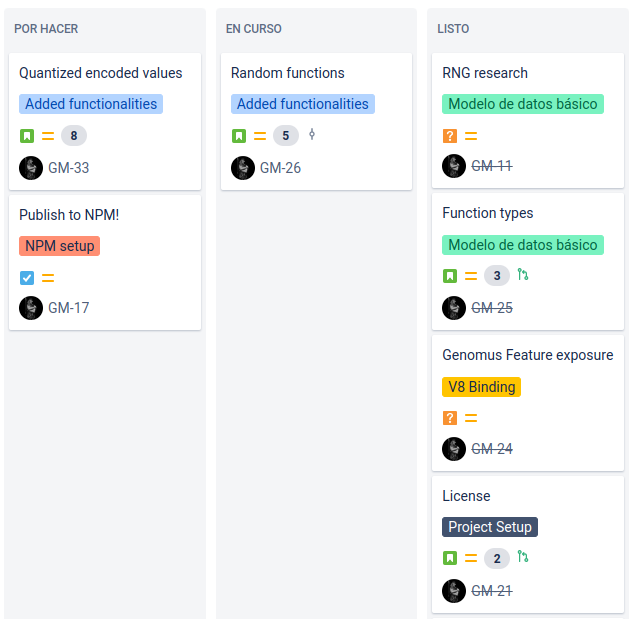
\includegraphics[width=\textwidth]{imagenes/kanban_04_07.png}
    \caption{Tablero KanBan del proyecto.} En su estado durante el último sprint, a fecha del 4 de julio de 2022.
    \label{fig:kanban_board}
\end{figure}

\subsubsection{Hitos e historias de usuario}

Las funcionalidades del MVP se han dividido en los siguientes hitos: 

\begin{itemize}
    \item \textit{Configuración del proyecto}. Hito en el que se han implementado las diferentes funcionalidades de despliegue del código y de control de versiones. Este hito ha incluido la configuración de los repositorios de git, la configuración del entorno de desarrollo y la creación de la integración circular.

    \item \textit{Modelo básico de datos}. Hito en el que se han implementado las funcionalidades más básicas para declarar genotipos y fenotipos, y realizar evaluaciones de genotipos.
    
    \item \textit{Funcionalidades añadidas}. Hito en el que se han incluidos las funcionalidades construidas sobre el modelo de datos. En este hito se incluyen el resto de transformaciones de datos, así como la representación de los datos como vectores numéricos normalizados.
        
    \item \textit{Enlace con V8}. Hito que ha incluido la investigación e implementación del enlace dinámico de nuestra librería compilada con el runtime de \verb|javascript|, que en este caso es el motor V8 al estar haciendo usode NodeJS\footnote{Más información en este artículo divulgativo de NodeJS sobre el motor V8: \url{https://nodejs.dev/learn/the-v8-javascript-engine}}.
    
    \item \textit{Publicación en NPM}. Hito que ha incluido la publicación del paquete \verb|genomus-core-js| en NPM.
\end{itemize}

Cada hito ha sido a su vez dividido en historias de usuario identificada de manera única por un código de historia. Al estar trabajando sobre el proyecto GenoMus, los códigos de historia siguen todos el formato \textit{GM-xxx}. En \ref{fig:roadmap} se puede ver como ha avanzado el progreso de los diferentes hitos, desglosado en historias de usuario individuales.

\begin{figure}
    \centering
    \centerline{
    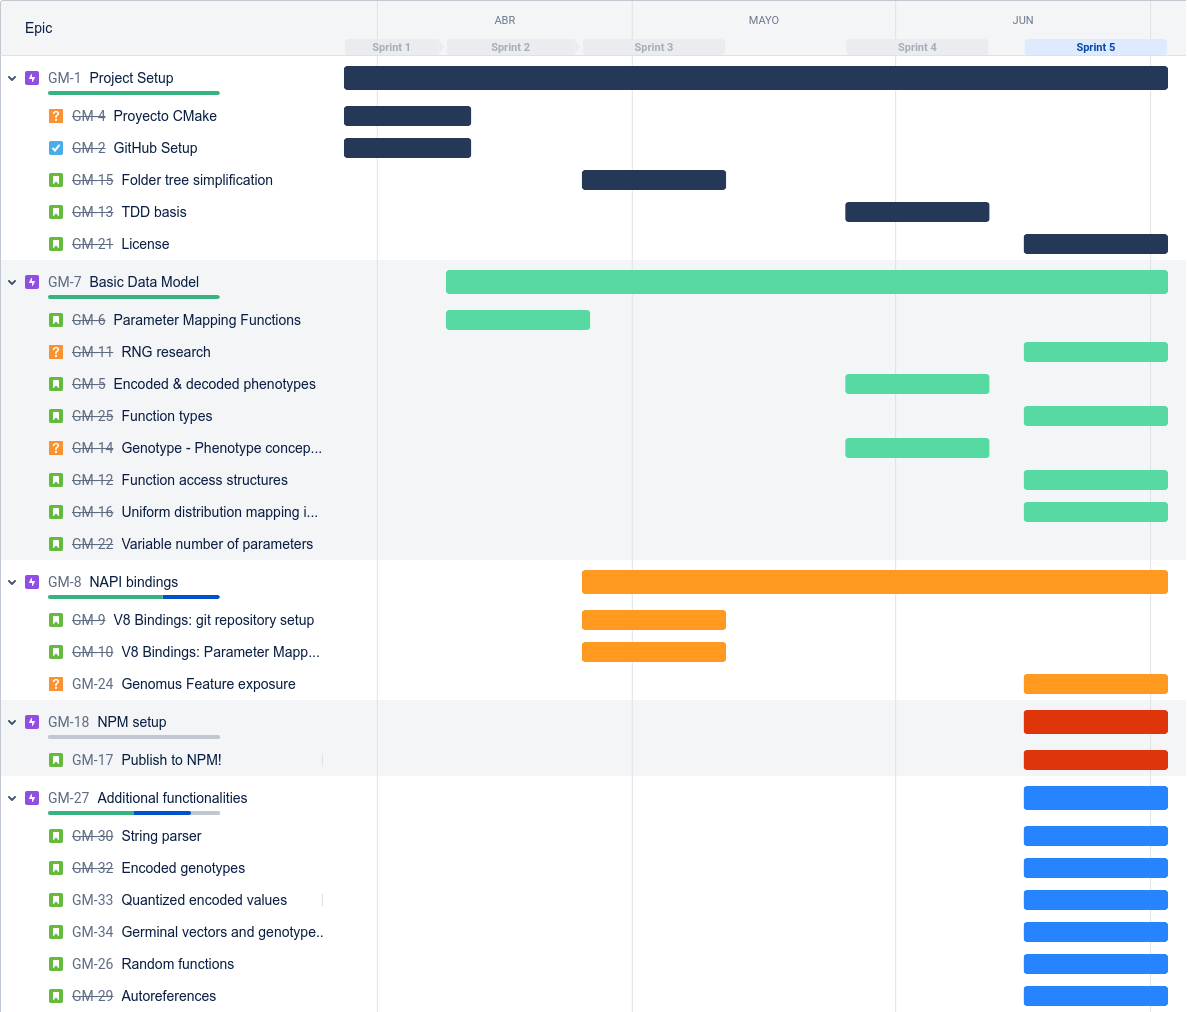
\includegraphics[width=0.8\paperwidth]{imagenes/road_map_03_07.png}
    }
    \caption{Hoja de ruta en proceso durante el sprint final del proyecto.}
    \label{fig:roadmap}
\end{figure}


\subsection{Protocolos de seguimiento del código}

Como se ha mencionado previamente, el proceso de desarrollo hace uso de un control de versiones con \verb|git| sobre repositorios alojados en Github y con una estructura de desarrollo que sigue un flujo de trabajo ampliamente inspirado en Gitflow. Se establecen los siguientes protocolos:

\subsubsection{Sobre ramas}

Las ramas utilizadas en el proyecto se clasifican en la rama principal \textit{master}, la rama de desarrollo \textit{develop} y las ramas de funcionalidad. Estas últimas están asociadas a una historia de usuario, cuyo código identificativo conforma el comienzo del nombre de la rama.

\subsubsection{Sobre mezclas}

La rama de desarrollo ramifica desde la rama principal, mientras que las ramas de funcionalidad ramifican desde la rama de desarrollo. Al finalizar una funcionalidad, la rama correspondiente se incorpora a la rama de desarrollo. Para realizar una \textit{release}, la rama de desarrollo se incorpora a la rama principal.
    
\subsubsection{Sobre peticiones de incorporación}

Las mezclas entre ramas estarán reflejadas en \textit{pull requests}, las cuales deberán tener un título descriptivo de las funcionalidades a incorporar y, opcionalmente, una descripción de estas. El único tipo de mezcla permitido en el proyecto es el \textit{squash and merge}\footnote{Refiriéndose a la funcionalidad de Github construida sobre el comando \textit{git merge --squash} consultable en la documentación oficial. \url{https://git-scm.com/docs/git-merge}}. Esto tiene el objetivo de mantener la limpieza de los \textit{logs}\footnote{Refiriéndose a los logs de git accesibles por el comando \textit{git log}. Más información en la documentación oficial de git. \url{https://www.git-scm.com/docs/git-log}} de las ramas de desarrollo y principal. Así, la rama de desarrollo solo registra un único \textit{commit} por historia de usuario, y la rama principal solo registra un commit por \textit{release}.
    
\subsubsection{Sobre tests automáticos}

La creación de una \textit{pull request} o el añadido de \textit{commits} a una rama observada por una \textit{pull request} debe disparar el lanzamiento de tests automáticos que comprueben la integridad de las funcionalidades previas a la rama. Idealmente se debe prohibir la incorporación de una rama con tests fallidos, pero esto es una funcionalidad que Github\footnote{Refiriéndose a la funcionalidad de \textit{reglas de protección de ramas} de Github. Consultable en la documentación oficial. \url{https://docs.github.com/en/repositories/configuring-branches-and-merges-in-your-repository/defining-the-mergeability-of-pull-requests/about-protected-branches}} no ofrece con su plan gratuíto, por lo que no se ha implementado.
    
\subsubsection{Sobre versionado semántico}

La publicación de una \textit{release} en la rama principal debe estar acompañada del etiquetado\footnote{Refiriéndose al etiquetado nativo de git, accesible a través del comando \textit{git tag} consultable en la documentación oficial. \url{https://git-scm.com/docs/git-tag}} de la rama principal con la versión del software a publicar.

	% Desarrollo bajo sprints: 
	% 	1. Permitir registros y login de usuarios
	% 	2. Desarrollo del sistema de incidencias
	% 	3. Desarrollo del sistema de denuncias administrativas y accidentes
	% 	4. Desarrollo del sistema de croquis
	%   5. Instalación de la aplicación de manera automática
	\chapter{Implementación}

Tras analizar el prototipo se propone la implementación de las funcionalidades y críticas de GenoMus en C++. Este subconjunto de las funcionalidades se desarrollará bajo el nombre de genomus-core. Se propone reutilizar las funcionalidades secundarias del prototipo de javascript. La totalidad del paquete se desarrollará bajo el nombre de genomus-js.

Así, la base de código se dividirá en tres áreas: (???)

\begin{enumerate} 
    \item Una librería de C++ que implementa el modelo de datos y de cómputo de GenoMus: genomus-core\cite{genomus-core}.
    \item Un módulo nativo de NodeJs (cita) que exponga una API de interación entre el runtime de JS y la biblioteca de C++: genomus-core-js\cite{genomus-core-js}.
    \item Un módulo de npm que encapsule lo previamente enunciado y reutilize la lógica de I/O del prototipo: genomus-js.
\end{enumerate}

\section{genomus-core}

\textbf{genomus-core} implementa el modelo de datos y de cómputo de GenoMus. 

\subsection{Modelo de datos}

Fácil

\subsection{Modelo de cómputo}
El modelo de cómputo de GenoMus está intrínsecamente basado en el paradigma de programación funcional. Esto hace que una implementación en C++ no sea trivial por diferentes motivos:

\begin{itemize}
    \item \textbf{Funciones dinámicas en tiempo de ejecución.} Las funciones de cómputo disponibles deben ser declarables en tiempo de ejecución. Ya que las funciones disponibles al modelo de cómputo son dependientes del estado del programa, es ideal que estas se puedan declarar dinámicamente en tiempo de ejecución. En la actual implementación, se proporciona una serie de funciones instanciadas en tiempo de carga.
    
    \item \textbf{Polimorfismo funcional.} Necesitamos construcciones que doten al modelo de cómputo de polimorfismo declarado en tiempo de ejecución. Debe ser posible no solo declarar nuevas funciones en tiempo de ejecución, sino también declarar nuevos tipos a usar como parámetros o salidas. Esto nos quita de la ecuación casi todos los constructos que C++ nos ofrece para conseguir polimorfismo dinámico, ya que el dominio del polimorfismo debe ser conocido en tiempo de compilación en C++. (cita requerida)
    
    \item \textbf{Árboles funcionales declarables y evaluables.} Toda instancia de cómputo debe no solo ser computable sino también almacenable. La instancia de árbol funcional debe existir independientemente de su evaluación. Así, una función de cómputo será un objeto invocable o functor cuya invocación contribuirá a la declaración del árbol funcional en memoria.
    
    (... ejemplo de código, diagrama de memoria(?))

    Esto, además de ser necesario para el funcionamiento del software, posibilita el diseño de algoritmos de cómputo sobre el árbol funcional más allá del típico recorrido por profundidad. (cita requerida - por ejemplo haskell graph reduction machine)
    
    \item \textbf{Funciones enumerables en tiempo de ejecución.} Las funciones de cómputo disponibles en tiempo de ejecución deben ser enumerables y referenciables según los diferentes métodos de acceso(cita a donde se explican las cosas codificadas/decodificadas).
\end{itemize}

Todas estas características son bien incompatibles con la metodología de desarrollo orientado a objetos estándar de C++ o bien incompatibles con la máxima del proyecto de ser asequible para programadores amateur, si pretendemos seguir las buenas prácticas de C++. Por este motivo se toma la decisión de alejarse de la práctica principal de polimorfismo funcional y de datos definida en los últimos estándares de C++ (C++11, C++17(cita requerida)) para realizar una implementación mixta entre orientada a objetos clásica y orientada a prototipos(cita requerida). 

Lo que nos aporta conceptualmente el diseño orientado a prototipos es la posibilidad de manejar parcialmente el tipado de nuestros objetos en tiempo de ejecución. Por otra parte, la principal desventaja que nos trae es la existencia de errores de tipado no conocidos por el compilador, lo cual es natural cuando lo que buscamos es precisamente declarar funciones de tipado arbitrario en tiempo de ejecución.

Así, se nos presenta un compromiso entre la seguridad del código y la legibilidad de este. La implementación propuesta busca maximizar la legibilidad y flexibilidad del código minimizando la cantidad de comprobaciones de tipado en tiempo de ejecución. Además, se plantea mitigar el riesgo del tipado dinámico mediante la creación de tests de integración.

\section{genomus-core-js}


	% Presupuesto

	% Conclusiones
	\chapter{Resultados}

\section{Mejoras de eficiencia respecto al prototipo}

Para validar la implementación realizada, se plantean una serie de mediciones comparativas entre instancias computacionales ejecutadas en el prototipo y en \verb|genomus-core| como estimación de las mejoras en eficiencia conseguidas a través de la implementación aportada. 

Se define una instancia de cómputo a realizar iterativamente durante diez segundos. Esta instancia de cómputo consiste en la creación de un vector germinal aleatorio\footnote{Refiriéndose a los vectores germinales descritos por GenoMus\cite{GenoMus-master}} sobre el cual se realizarán las siguientes transformaciones, todas ellas descritas de la misma manera por GenoMus:

\begin{itemize}
    \item Normalización del vector para representar un genotipo válido.
    \item Transformación del vector normalizado a una expresión en forma de texto.
    \item Obtención de un árbol genotípico o genotipo decodificado a través del parser con la expresión como entrada.
    \item Evaluación del genotipo decodificado en un fenotipo codificado.
    \item Representación del fenotipo codificado como un vector numérico.
\end{itemize}

En términos del prototipo, esta serie de evaluaciones y transformaciones son equivalentes a una llamada a la función \verb|createGenotype|. Las instancias de cómputo en ambos software estarán afectadas por los siguientes parámetros:

\begin{itemize}
    \item \textbf{Funciones de GenoMus a utilizar.} Las funciones GenoMus utilizadas tanto por el prototipo como por \verb|genomus-core| son la intersección de funciones definidas en un software y en otro, asegurando así la equivalencia en coste computacional de las instancias de código. La lista de funciones implementadas utilizada se puede consultar en la tabla \ref{tab:used_functions}.
    
    \item \textbf{Longitud máxima del vector germinal.} Se define una longitud máxima del vector germinal de 256.
    \item \textbf{Tamaño máximo por defecto de listas.} Se define un tamaño por defecto de listas de 256.
    \item \textbf{Profundidad máxima de anidamiento de funciones.} Se define una profundidad máxima de anidamiento de 256.
\end{itemize}

\begin{table}[]
    \centering
    \begin{tabular}{p{4cm} p{5cm}}
        Tipo de salida & Funciones \\ \hline \hline
        eventF & e\_piano, eAutoref \\ \hline
        voiceF & v, vConcatE, vConcatV, vMotif, vMotifLoop, vPerpetuumMobile, vPerpetuumMobileLoop, vAutoref \\ \hline
        scoreF & s, sAddV, sAddS \\ \hline
        noteValueF & n, nRnd \\ \hline
        midiPitchF & m, mRnd \\ \hline
        durationF & d, dRnd \\ \hline
        frequencyF & f, fRnd \\ \hline
        articulationF & a, aRnd \\ \hline
        intensityF & i, iRnd \\ \hline
        quantizedF & q, qRnd \\ \hline
        goldenIntegerF & z, zRnd \\ \hline
        lnoteValueF & ln \\ \hline
        lmidiPitchF & lm \\ \hline
        ldurationF & ld \\ \hline
        lfrequencyF & lf \\ \hline
        larticulationF & la \\ \hline
        lintensityF & li \\ \hline
    \end{tabular}
    \caption{Funciones GenoMus utilizadas en las pruebas de eficiencia.} Las descripciones de estas funciones pueden ser encontradas en las especificaciones de GenoMus\cite{GenoMus}. La implementación exacta de estas en \verb|genomus-core| se puede encontrar en el archivo \textit{function\_library.cpp} del repositorio.
    \label{tab:used_functions}
\end{table}

En la tabla \ref{tab:datos_entorno_test} se puede ver una especificación de las características de la máquina donde se ha llevado a cabo la ejecución. Podemos anotar que tanto el prototipo\footnote{
    NodeJS es monohebra a pesar de soportar programación asíncrona. Más información sobre el ciclo de eventos de NodeJS en el siguiente artículo. \url{https://nodejs.org/en/docs/guides/event-loop-timers-and-nexttick/}
} como \verb|genomus-core| no hacen uso de procesamiento paralelo, por lo que la ejecución recae sobre un solo núcleo en cada instante de tiempo.

Como podemos observar en los resultados obtenidos, expuestos en la tabla \ref{tab:resultados_benchmark}, podemos decir que \verb|genomus-core| es aproximadamente cinco veces más rápido que GenoMus en este tipo de instancia de cómputo. Así, se puede decir que el proyecto cumple su objetivo principal. Estos benchmarks han sido ejecutados sobre el MVP de \verb|genomus-core|, por lo que también se puede pensar que hay todavía mucho espacio para la optimización del software.

\begin{table}[]
    \centering
    \begin{tabular}{p{4cm} p{7cm}}
        \textbf{CPU} &  \\ \hline \hline
        Modelo & Intel(R) Core(TM) M-5Y10c CPU \\ 
        Arquitectura & x86\_64 \\
        Núcleos físicos & 2 \\
        Núcleos lógicos & 4 \\
        & \\
        \textbf{Sistema Operativo} & \\ \hline \hline
        Distribución & Ubuntu 20.04.4 LTS x86\_64 \\
        Kernel & linux 5.4.0-121-generic \\
        & \\        
        \textbf{NodeJS} & \\ \hline \hline
        Versión de NodeJS & v16.0.0 \\
        & \\
        \textbf{C++} & \\ \hline \hline
        Compilador & g++ (gcc) \\
        Versión & 9.4.0 (Ubuntu 9.4.0-1ubuntu1~20.04.1) \\
        Nivel de optimización & CMAKE\_CXX\_FLAGS\_RELEASE \\
        & (-O3 en gcc)
        
    \end{tabular}
    \caption{Especificaciones del entorno de ejecución.}
    \label{tab:datos_entorno_test}
\end{table}

\begin{table}[h]
    \begin{subtable}[h]{0.45\textwidth}
        \centering
        \begin{tabular}{p{1.5cm} p{1cm} p{1.8cm}}
            t (ms) & i & t\_avg (ms) \\ \hline \hline
            
            10633 & 48 & 221,52 \\ 
            10194 & 62 & 164,42 \\ 
            10554 & 79 & 133,59 \\ 
            13221 & 46 & 287,41 \\ 
            14195 & 57 & 249,04 \\ 
            20244 & 12 & 1687 \\ 
            10011 & 39 & 256,69 \\ 
            10937 & 56 & 195,30 \\ \hline
            99989 & 399 & 250,60 \\ 
            
        \end{tabular}
       \caption{GenoMus}
       \label{tab:genomus_benchmark}
    \end{subtable}
    \hfill
    \begin{subtable}[h]{0.45\textwidth}
        \centering
        \begin{tabular}{p{1.5cm} p{1cm} p{1.8cm}}
            t (ms) & i & t\_avg (ms) \\ \hline \hline
            10014 & 176 & 56,90 \\ 
            10056 & 210 & 47,89 \\ 
            10436 & 284 & 36,75 \\ 
            11393 & 160 & 71,21 \\ 
            11452 & 110 & 104,11 \\ 
            10080 & 216 & 46,67 \\ 
            10081 & 288 & 35,00 \\ 
            12145 & 259 & 46,89 \\ \hline
            85657 & 1703 & 50,30 \\ 
        \end{tabular}
       \caption{genomus-core}
       \label{tab:genomus-core_benchmark}
     \end{subtable}
     \caption{Resultados del benchmark.} Podemos ver dos tablas conteniendo respectivamente los resultados del benchmark para GenoMus y \verb|genomus-core|. Las columnas tienen los siguientes significados: \textit{t} representa el tiempo total de computación, \textit{i} representa el número total de iteraciones completadas y \textit{t\_avg} representa el tiempo medio por iteración. La última fila de cada tabla corresponde con los resultados totales a lo largo de las ocho ejecuciones del benchmark para cada software.
     \label{tab:resultados_benchmark}
\end{table}

\section{Completitud del MVP}

En el ámbito de gestión del proyecto, se puede decir que el proceso de desarrollo ha sido exitoso, ya que se ha podido completar el MVP que se buscaba para la fecha prevista. En la figura \ref{fig:jira_num_issues} podemos ver cómo el progreso de historias completadas sigue la pendiente usual de un proyecto de estas características.

\begin{figure}
    \centering
    \centerline{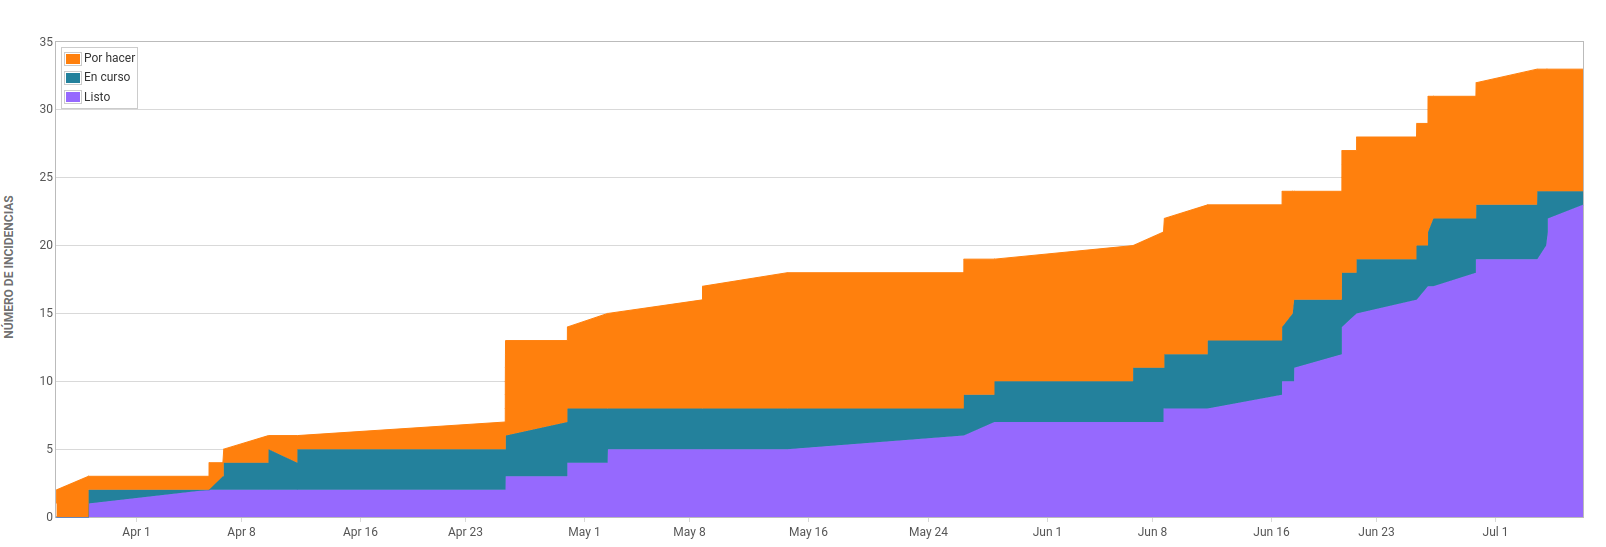
\includegraphics[width=0.8\paperwidth]{imagenes/jira_num_issues.png}}
    \caption{Diagrama de flujo acumulado del progreso en el desarrollo de historias de usuario.} En este diagrama podemos analizar el progreso del desarrollo de las historias de usuario. Las historias no completadas corresponden a funcionalidades no incluidas en el MVP, por lo que quedan pendientes como trabajo futuro.
    \label{fig:jira_num_issues}
\end{figure}
	

	% Trabajos futuros
	\chapter{Trabajos futuros}


Como se ha explicado en el capítulo \ref{cap:implementacion}, la implementación del paquete \verb|genomus-js| no ha sido incluida en este proyecto fin de grado. Por este motivo, el principal trabajo a realizar tras la clausura de este proyecto es la implementación de las funcionalidades de \verb|genomus-js|, ya sea mediante un total rediseño de las funcionalidades o mediante la reutilización de código del prototipo. En este paquete se incluirían funcionalidades como:

\begin{itemize}
    \item Integración con los distintos software de terceros que conforman las interfaces de usuario de GenoMus.
    \item Funcionalidades de alto nivel como la creación de genotipos basados en características del fenotipo que producen.
    \item Un corpus completo de funciones GenoMus.
\end{itemize}

Por otra parte, tras la finalización de este proyecto fin de grado también se da la posibilidad de realizar un proceso de optimización del código implementado. Debido a las dificultades de desarrollo expuestas en la sección \ref{ssec:dificultades}, se presentan diferentes procedimientos cuyo rendimiento es mejorable. Tras analizar los diferentes ejecutables con \verb|gprof|, se puede ver que los ejecutables realizan una gran cantidad de copias innecesarias de datos, las cuales podrían ser probablemente evitadas mediante el uso de referencias en más lugares del código. Otro planteamiento posible sería la introducción de procesamiento paralelo en el motor de cómputo.

    % Conclusiones
	\chapter{Conclusiones}

Tras la finalización de este trabajo de fin de grado puedo reconocer haber obtenido una serie de conocimientos acerca de los fundamentos técnicos proyecto GenoMus que me han permitido realizar una aportación con la que me hallo satisfecho. Considero que el trabajo realizado puede mejorar la calidad y robustez de GenoMus como proyecto de software libre, lo cual ha sido el objetivo desde el principio como se ha reflejado en la sección \ref{motivacion}.
\\ \\
Pienso que el trabajo reflejado en este documento me ha hecho más consciente del abanico de posibilidades técnicas de la evolución futura del proyecto, y en consecuencia también de las posibilidades prácticas que esto conlleva. El éxito del modelo de cómputo desarrollado posibilita la clausura de este primer proceso de contribución y permite mirar al frente hacia el trabajo futuro.
\\ \\
En el ámbito del fin de mi formación como estudiante del Grado de Ingeniería Informática puedo decir que considero que este trabajo ha constituido un episodio muy fructífero de mi formación. Considero que me he adentrado en campos que han ensanchado mi perspectiva no solo sobre el proyecto GenoMus, sino también sobre conceptos de las ciencias de la computación como gramáticas o compiladores y de la ingeniería del software como las arquitecturas heterogéneas, la gestión de proyectos o el software libre. 
	
	\newpage
	\bibliography{bibliografia}
	\bibliographystyle{plain}
	
\end{document}

